\section{Experiment}

\subsection{Datasets}
{\bf ICVL Hand Posture Dataset.} 
The ICVL dataset~\cite{tang2014latent} consists of 330K training and 1.6K testing depth images. The frames are collected from 10 different subjects using Intel's Creative Interactive Gesture Camera~\cite{melax2013dynamics}. The annotation of hand pose contains 16 joints, which include three joints for each finger and one joint for the palm.

{\bf NYU Hand Pose Dataset.}
The NYU dataset~\cite{tompson2014real} consists of 72K training and 8.2K testing depth images. The training set is collected from subject A, whereas the testing set is collected from subjects A and B by three Kinects from different views. The annotations of hand pose contain 36 joints. Most of the previous works only used frames from the frontal view and 14 out of 36 joints in the evaluation, and we also followed them.

{\bf MSRA Hand Pose Dataset.}
The MSRA dataset~\cite{sun2015cascaded} contains 9 subjects with 17 gestures for each subject. Intel's Creative Interactive Gesture Camera~\cite{melax2013dynamics} captured 76K depth images with 21 annotated joints. For evaluation, the leave-one-subject-out cross-validation strategy is utilized. 

{\bf HANDS 2017 Frame-based 3D Hand Pose Estimation Challenge Dataset.}
The HANDS 2017 frame-based 3D hand pose estimation challenge dataset~\cite{yuan20172017} consists of 957K training and 295K testing depth images that are sampled from BigHand2.2M~\cite{Yuan_2017_CVPR} and First-Person Hand Action~\cite{garcia2017first} datasets. There are five subjects in the training set and ten subjects in the testing stage, including five unseen subjects. The ground-truth of this dataset is the 3D coordinates of 21 hand joints.

{\bf ITOP Human Pose Dataset.}
The ITOP dataset~\cite{haque2016towards} consists of 40K training and 10K testing depth images for each of the front-view and top-view tracks. This dataset contains depth images with 20 actors who perform 15 sequences each and is recorded by two Asus Xtion Pro cameras. The ground-truth of this dataset is the 3D coordinates of 15 body joints.


\subsection{Evaluation metrics}

We used 3D distance error and percentage of success frame metrics for 3D hand pose estimation following~\cite{tang2014latent,sun2015cascaded}. For 3D human pose estimation, we used mean average precision (mAP) that is defined as the detected ratio of all human body joints based on 10 cm rule following~\cite{haque2016towards,yub2015random}.

\subsection{Ablation study}
We used NYU hand pose dataset~\cite{tompson2014real} to analyze each component of our model because this dataset is challenging and far from saturated.

\begin{table}[]
\centering
\setlength\tabcolsep{1.0pt}
\def\arraystretch{1.1}
\begin{tabular}{L{2.6cm}|C{2.5cm}C{3cm}}
\specialrule{.1em}{.05em}{.05em} 
   Input \textbackslash Output & 3D Coordinates & Per-voxel likelihood  \\ \hline
2D depth map & 18.85 (21.1 M) & 13.01 (4.6 M) \\ 
3D voxelized grid & 16.78 (457.5 M)  & \textbf{10.37 (3.4 M)} \\ \specialrule{.1em}{.05em}{.05em} 
\end{tabular}
\vspace*{-3mm}
\caption{Average 3D distance error (mm) and number of parameter comparison of the input and output types in the NYU dataset. The number in the parenthesis denotes the number of parameters. The visualized model for each input and output type is shown in Figure~\ref{fig:comparison_io_type}.}
\label{table:nyu_io_type}
\end{table}

\begin{table}
\centering
\setlength\tabcolsep{1.0pt}
\def\arraystretch{1.1}
\begin{tabular}{L{3.7cm}C{3.7cm}}
\specialrule{.1em}{.05em}{.05em} 
   Methods  &  Average 3D distance error \\ \hline
Baseline      & 11.14 mm \\ 
 + Localization refinement      &  9.22 mm \\ 
 + Epoch ensemble      & 8.42 mm \\ \specialrule{.1em}{.05em}{.05em}
\end{tabular}
\vspace*{-3mm}
\caption{Effect of localization refinement and epoch ensemble. The average 3D distance error is calculated in the NYU dataset.}
\vspace*{-4mm}
\label{table:nyu_R_E}
\end{table}

\begin{figure*}
\begin{center}
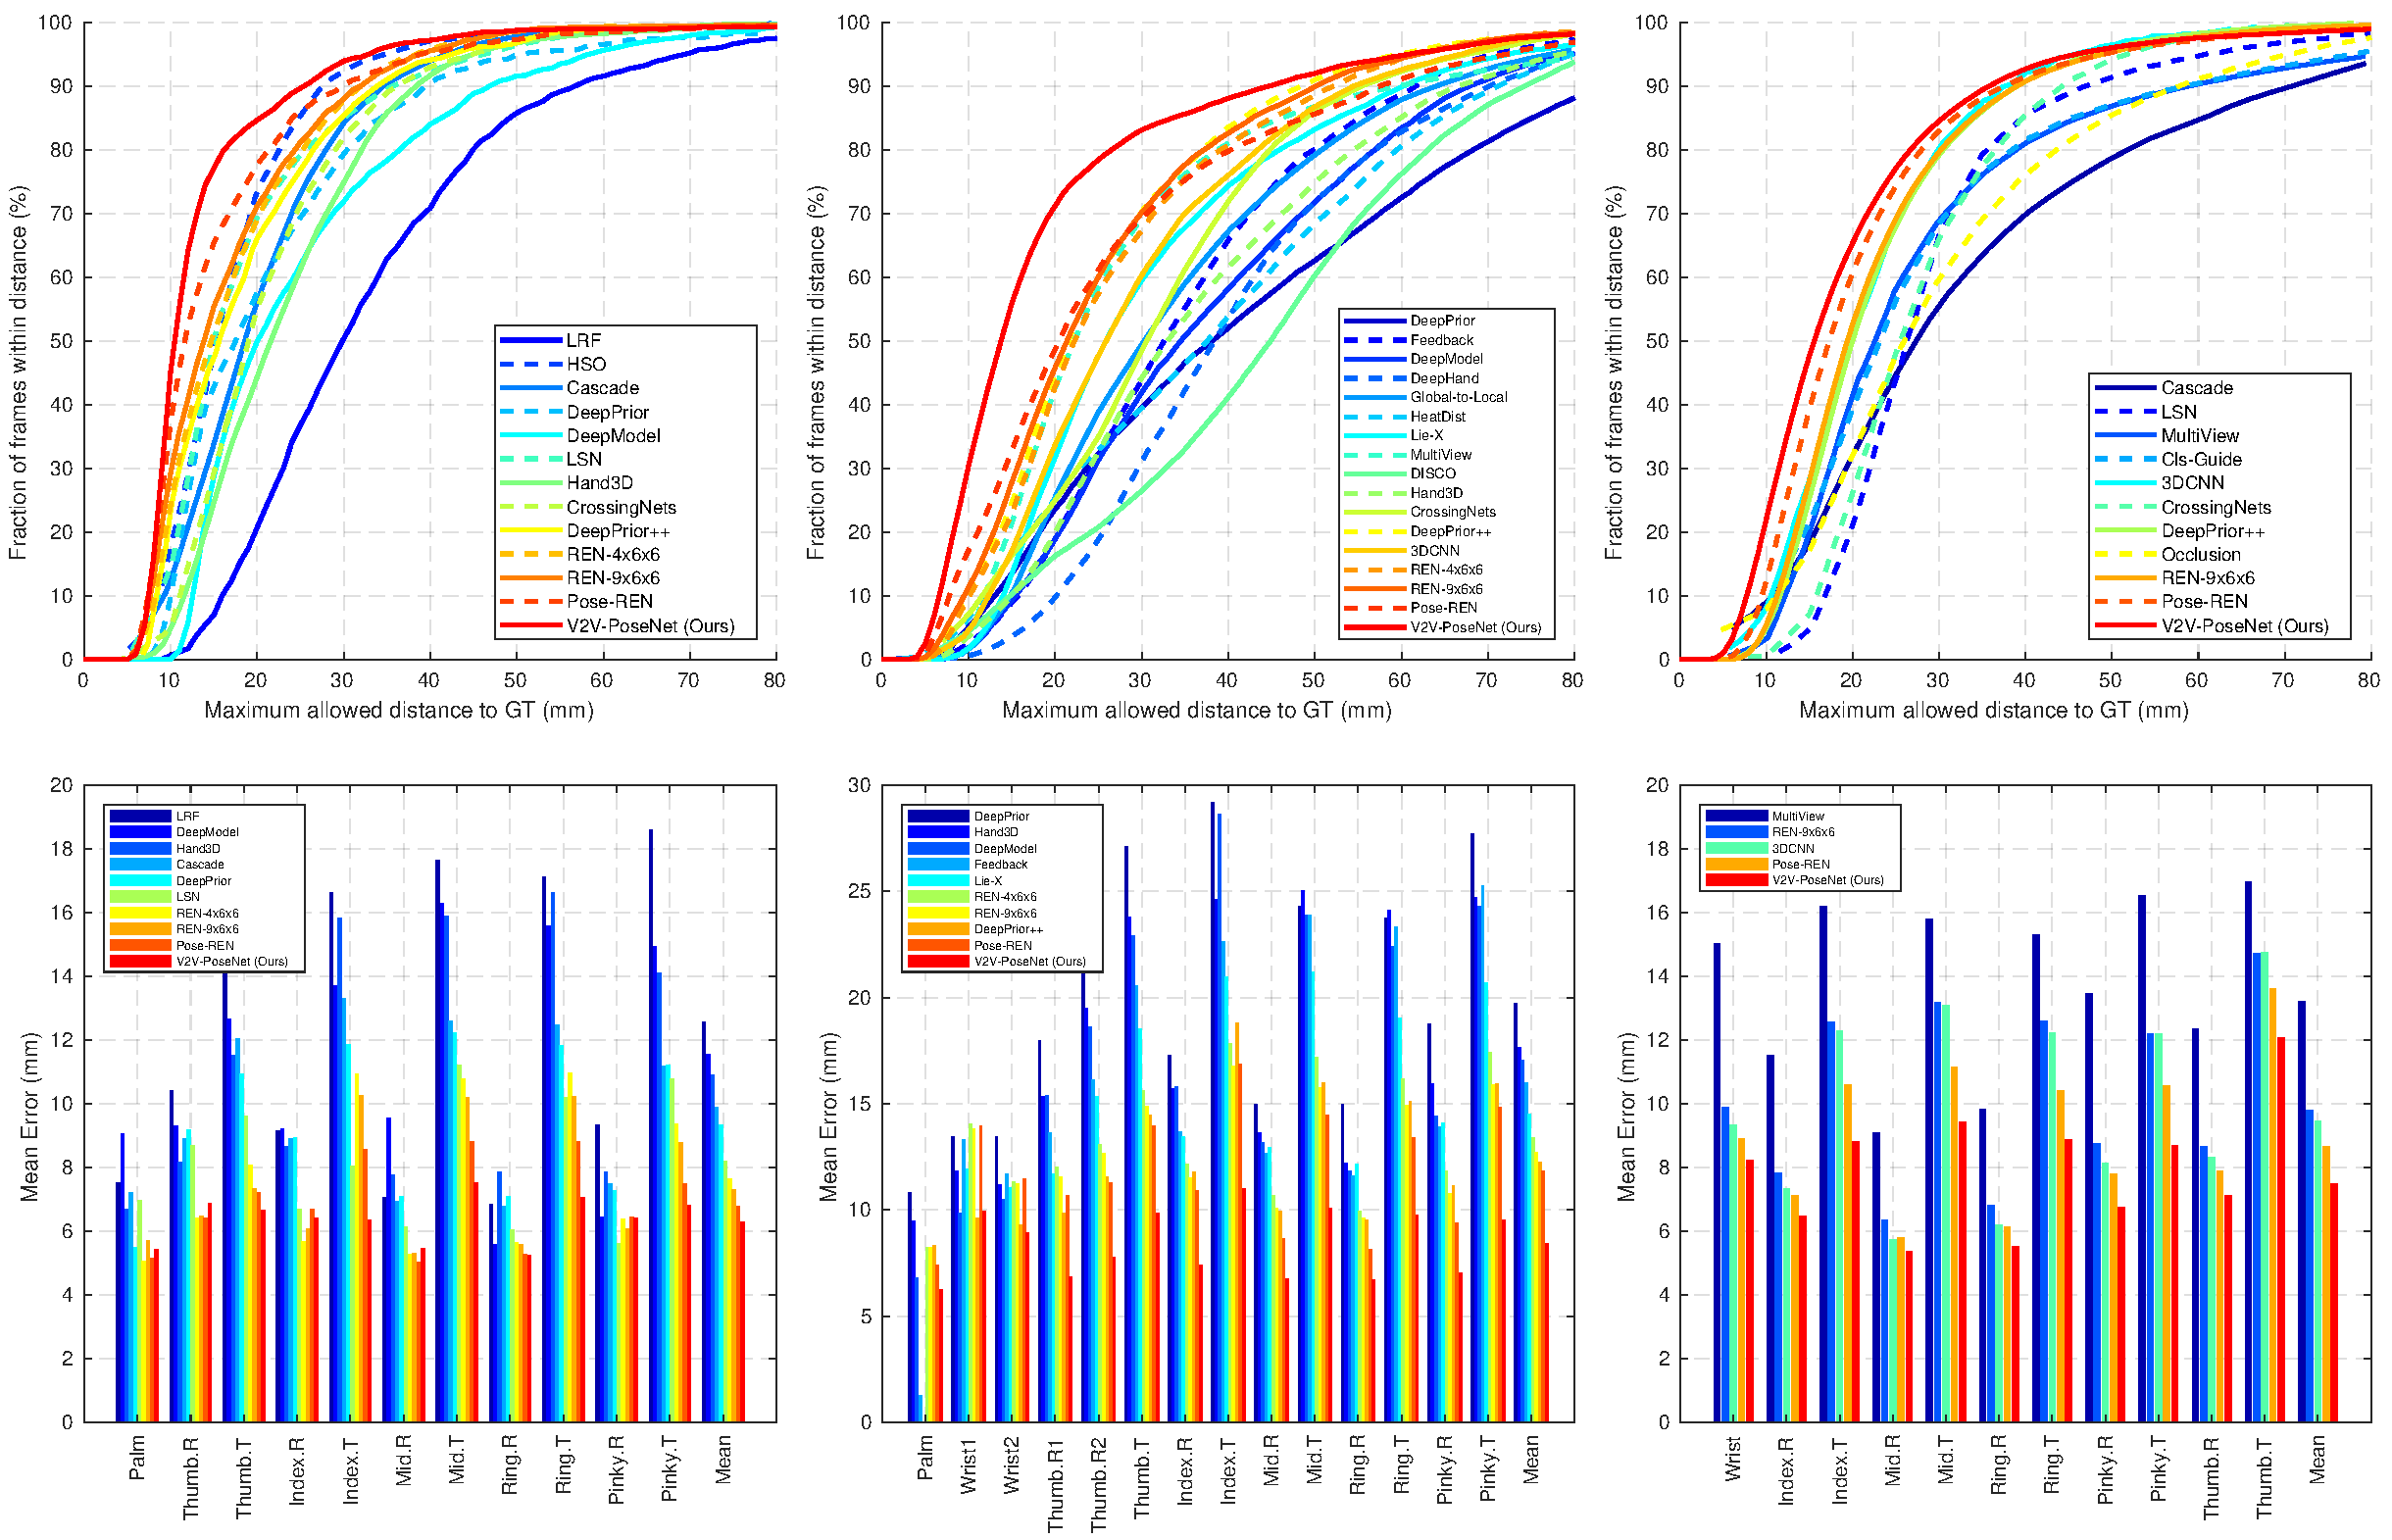
\includegraphics[width=1.0\linewidth]{comparison_with_stoa.pdf}
\end{center}
\vspace*{-5mm}
   \caption{Comparison of the proposed method (V2V-PoseNet) with state-of-the-art methods. Top row: the percentage of success frames over different error thresholds. Bottom row: 3D distance errors per hand keypoints. Left: ICVL dataset, middle: NYU dataset, right: MSRA dataset.}
\label{fig:comparison_with_stoa}
\end{figure*}

\begin{figure}[t]
\begin{center}
   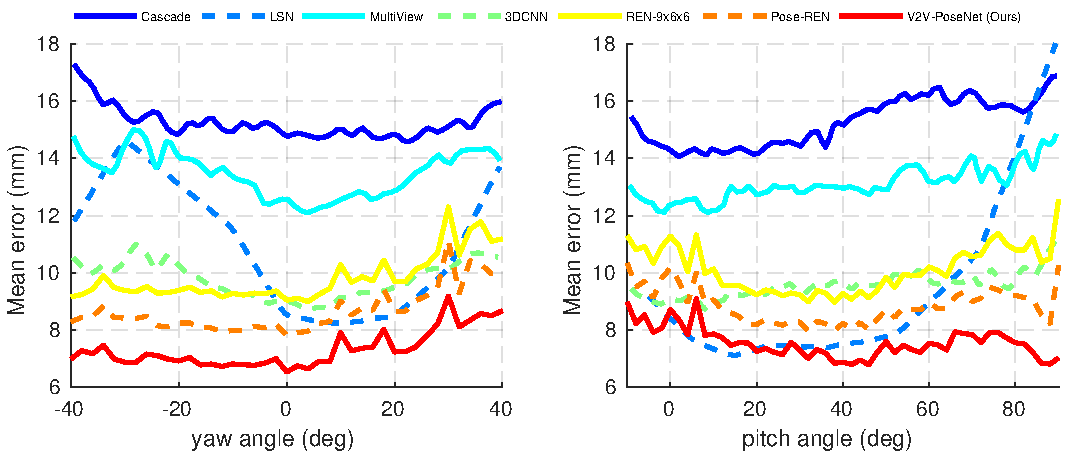
\includegraphics[width=1.0\linewidth]{msra_yaw_pitch.pdf}
\end{center}
\vspace*{-5mm}
   \caption{Comparison of average 3D distance error over different yaw (left) and pitch (right) angles on the MSRA dataset.}
\vspace*{-3mm}
\label{fig:msra_yaw_pitch}
\end{figure}


\begin{table*}[t]
\centering
\setlength\tabcolsep{1.0pt}
\def\arraystretch{1.1}
\begin{subtable}[t]{.34\textwidth}
\centering
\begin{tabular}[t]{C{3.1cm}C{2.5cm}}
\specialrule{.1em}{.05em}{.05em} 
   Methods  &  Mean error (mm)  \\ \hline
LRF     & 12.58  \\ 
DeepModel     &  11.56 \\ 
Hand3D     &  10.9  \\ 
CDO & 10.5 \\
DeepPrior      & 10.4  \\ 
CrossingNets    &  10.2  \\ 
Cascade      & 9.9  \\
JTSC    &  9.16  \\ 
DeepPrior++      &  8.1  \\ 
REN-4x6x6	& 7.63 \\
REN-9x6x6      &  7.31  \\ 
Pose-REN     &  6.79  \\
\textbf{V2V-PoseNet (Ours)}      &  \textbf{6.28}  \\ \specialrule{.1em}{.05em}{.05em} 
\end{tabular}
\caption{ICVL}
\end{subtable}%
\begin{subtable}[t]{.34\textwidth}
\centering
\begin{tabular}[t]{C{3.1cm}C{2.5cm}}
\specialrule{.1em}{.05em}{.05em} 
   Methods  &  Mean error (mm)  \\ \hline
DISCO & 20.7\\
DeepPrior     & 19.73  \\ 
Hand3D     &  17.6 \\ 
DeepModel    &  17.04  \\ 
JTSC    &  16.8  \\ 
Feedback     &  15.97  \\ 
Global-to-Local     &  15.60  \\ 
Lie-X      &  14.51  \\ 
3DCNN     &  14.1  \\ 
REN-4x6x6	& 13.39 \\
REN-9x6x6    &  12.69  \\ 
DeepPrior++      &  12.24  \\ 
Pose-REN     &  11.81  \\
\textbf{V2V-PoseNet (Ours)}      &  \textbf{8.42}  \\ \specialrule{.1em}{.05em}{.05em} 
\end{tabular}
\caption{NYU}
\end{subtable}%
\begin{subtable}[t]{.34\textwidth}
\centering
\begin{tabular}[t]{C{3.1cm}C{2.5cm}}
\specialrule{.1em}{.05em}{.05em} 
   Methods  &  Mean error (mm)  \\ \hline
Cascade     & 15.2  \\
Cls-Guide& 13.7 \\
MultiView    & 13.2  \\
Occlusion    & 12.8  \\
CrossingNets     &  12.2  \\  
REN-9x6x6     &  9.7  \\ 
DeepPrior++      &  9.5 \\ 
Pose-REN     &  8.65  \\
\textbf{V2V-PoseNet (Ours)}      &  \textbf{7.49}  \\ \specialrule{.1em}{.05em}{.05em} 
\end{tabular}
\caption{MSRA}
\end{subtable}%
\caption{Comparison of the proposed method (V2V-PoseNet) with state-of-the-art methods on the three 3D hand pose datasets. Mean error indicates the average 3D distance error.}
\vspace*{-3mm}
\label{table:comparison_with_stoa}
\end{table*}


{\bf 3D representation and per-voxel likelihood estimation.}
To demonstrate the validity of the 3D representation of the input and per-voxel likelihood estimation, we compared the performances of the four different combinations of the input and output forms in Table~\ref{table:nyu_io_type}. As the table shows, converting the input representation type from the 2D depth map to 3D voxelized form (also converting the model from 2D CNN to 3D CNN) substantially improves performance, regardless of output representation. This justifies the effectiveness of the proposed 3D input representation that is free from perspective distortion. The results also show that converting the output representation from the 3D coordinates to the per-voxel likelihood increases the performance significantly, regardless of the input type. Among the four combinations, \emph{voxel-to-voxel} gives the best performance even with the smallest number of parameters. Hence, the superiority of the \emph{voxel-to-voxel} prediction scheme compared with other input and output combinations is clearly justified. 


To fairly compare four combinations, we used the same network building blocks and design, which were introduced in Section~\ref{V2V-PoseNet_Section}. The only difference is that the model for the per-voxel likelihood estimation is fully convolutional, whereas for the coordinate regression, we used fully connected layers at the end of the network. Simply converting \emph{voxel-to-voxel} to \emph{pixel-to-voxel} decreases the number of parameters because the model is changed from the 3D CNN to the 2D CNN. To compensate for this change, we doubled the number of channels of each feature map in the \emph{pixel-to-voxel} model. If the number of channels is not doubled, then the performance was degraded. For all four models, we used 48$\times$48 depth map or 48$\times$48$\times$48 voxelized grid as input because the original size (88$\times$88$\times$88) does not fit into GPU memory in the case of \emph{voxel-to-coordinates}.


{\bf Refining localization of the target object.}
To demonstrate the importance of the localization refining procedure in Section~\ref{refineRefPoint_Section}, we compared the performance of two with and without the localization refinement step. As shown in Table~\ref{table:nyu_R_E}, the refined reference points significantly boost the accuracy of our model, which shows that the reference point refining procedure has a crucial influence on the performance.


{\bf Epoch ensemble.}
To obtain more accurate and robust estimation, we applied a simple ensemble technique that we call \emph{epoch ensemble}. The epoch ensemble averages the estimations from several epochs. Specifically, we save the trained model for each epoch in the training stage and then in the testing stage, we average all the estimated 3D coordinates from the trained models. As we trained our model by 10 epochs, we used 10 models to obtain the final estimation. Epoch ensemble has no influence in running time when each model is running in different GPUs. However, in a single-GPU environment, epoch ensemble linearly increases running time. The effect of epoch ensemble is shown in Table~\ref{table:nyu_R_E}.


\subsection{Comparison with state-of-the-art methods}
We compared the performance of the V2V-PoseNet on the three 3D hand pose estimation datasets (ICVL~\cite{tang2014latent}, NYU~\cite{tompson2014real}, and MSRA~\cite{sun2015cascaded}) with most of the state-of-the-art methods, which include latent random forest (LRF)~\cite{tang2014latent}, cascaded hand pose regression (Cascade)~\cite{sun2015cascaded}, DeepPrior with refinement (DeepPrior)~\cite{oberweger2015hands}, feedback loop training method (Feedback)~\cite{oberweger2015training}, hand model based method (DeepModel)~\cite{zhou2016model}, hierarchical sampling optimization (HSO)~\cite{tang2015opening}, local surface normals (LSN)~\cite{wan2016hand}, multi-view CNN (MultiView)~\cite{ge2016robust}, DISCO~\cite{bouchacourt2016disco}, Hand3D~\cite{deng2017hand3d}, DeepHand~\cite{sinha2016deephand}, lie-x group based method (Lie-X)~\cite{xu2017lie}, improved DeepPrior (DeepPrior++)~\cite{Oberweger_2017_ICCV_Workshops}, region ensemble network (REN-4$\times$6$\times$6~\cite{guo2017ren}, REN-9$\times$6$\times$6~\cite{guo2017towards}), CrossingNets~\cite{Wan_2017_CVPR}, pose-guided REN (Pose-REN)~\cite{chen2017pose}, global-to-local prediction method (Global-to-Local)~\cite{madadi2017end}, classification-guided approach (Cls-Guide)~\cite{yang2016hand}, 3DCNN based method (3DCNN)~\cite{ge20173d},  occlusion aware based method (Occlusion)~\cite{madadi2017occlusion}, and hallucinating heat distribution method (HeatDist)~\cite{Choi_2017_ICCV}. Some reported results of previous works~\cite{tang2014latent,oberweger2015hands,oberweger2015training,zhou2016model,Oberweger_2017_ICCV_Workshops,guo2017ren,guo2017towards,chen2017pose,xu2017lie} are calculated by prediction labels available online. Other results~\cite{sun2015cascaded,tang2015opening,wan2016hand,sinha2016deephand,ge2016robust,deng2017hand3d,Wan_2017_CVPR,madadi2017end,ge20173d,madadi2017occlusion,Choi_2017_ICCV,bouchacourt2016disco,yang2016hand} are calculated from the figures and tables of their papers.

\begin{table}
\centering
\setlength\tabcolsep{1.0pt}
\def\arraystretch{1.1}
\begin{tabular}{L{4.5cm}C{3.7cm}}
\specialrule{.1em}{.05em}{.05em} 
   Team name &  Average 3D distance error \\ \hline
V2V-PoseNet (Ours)      & \textbf{9.95 mm} \\ 
NVResearch and UMontreal      &  10.18 mm \\ 
NTU     & 11.30 mm \\ 
THU VCLab      & 11.70 mm \\ 
NAIST RVLab      & 11.90 mm \\ \specialrule{.1em}{.05em}{.05em}
\end{tabular}
\vspace*{-3mm}
\caption{The top-5 results of the HANDS 2017 frame-based 3D hand pose estimation challenge.}
\vspace*{-5.5mm}
\label{table:hands2017_result}
\end{table}

\begin{table*}
\centering
\setlength\tabcolsep{1.0pt}
\def\arraystretch{1.1}
\begin{tabular}{L{1.5cm}|C{1.0cm}C{1.1cm}C{1.1cm}C{1.0cm}C{1.2cm}C{2.0cm}|C{1.0cm}C{1.1cm}C{1.1cm}C{1.0cm}C{1.2cm}C{2.0cm}}
\specialrule{.1em}{.05em}{.05em} 
 & \multicolumn{6}{c|}{mAP (front-view)}  &  \multicolumn{6}{c}{mAP (top-view)} \\ \hline
   Body part & RF & RTW & IEF &VI & REN-9x6x6 & V2V-PoseNet (Ours)  & RF & RTW & IEF & VI & REN-9x6x6 & V2V-PoseNet (Ours) \\ \hline
Head & 63.8 & 97.8 & 96.2 & 98.1 & \textbf{98.7} & 98.29 & 95.4 & \textbf{98.4} & 83.8 & 98.1 & 98.2 & \textbf{98.4} \\ 
Neck & 86.4 & 95.8 & 85.2 & 97.5 & \textbf{99.4} & 99.07 & 98.5 & 82.2 & 50.0 & 97.6 & 98.9 & \textbf{98.91} \\ 
Shoulders & 83.3 & 94.1 & 77.2 & 96.5 & 96.1 & \textbf{97.18} & 89.0 & 91.8 & 67.3 & 96.1 & 96.6 & \textbf{96.87} \\ 
Elbows & 73.2 & 77.9 & 45.4 &  73.3 & 74.7 & \textbf{80.42} & 57.4 & 80.1 & 40.2 & \textbf{86.2} & 74.4 & 79.16 \\ 
Hands & 51.3 & \textbf{70.5} & 30.9 & 68.7 & 55.2 & 67.26 & 49.1 & 76.9 & 39.0 & \textbf{85.5} & 50.7 & 62.44\\ 
Torso & 65.0 & 93.8 & 84.7 & 85.6 & 98.7 & \textbf{98.73} & 80.5 & 68.2 & 30.5 & 72.9 & \textbf{98.1} & 97.78 \\ 
Hip & 50.8 & 80.3 & 83.5 & 72.0 & 91.8 & \textbf{93.23} & 20.0 & 55.7 & 38.9 & 61.2 & 85.5 & \textbf{86.91}\\ 
Knees & 65.7 & 68.8 & 81.8 & 69.0 & 89.0 & \textbf{91.80} & 2.6 & 53.9 & 54.0 & 51.6 & 70.0 & \textbf{83.28}\\ 
Feet & 61.3 & 68.4 & 80.9 & 60.8 & 81.1 & \textbf{87.6} & 0.0 & 28.7 & 62.4 & 51.5 & 41.6 & \textbf{69.62}\\ \hhline{-------------}
Mean & 65.8 & 80.5 & 71.0 & 77.4 & 84.9 & \textbf{88.74} & 47.4 & 68.2 & 51.2 & 75.5 & 75.5 & \textbf{83.44}\\ \specialrule{.1em}{.05em}{.05em} 
\end{tabular}
\vspace*{-3mm}
\caption{Comparison of the proposed method (V2V-PoseNet) with state-of-the-art methods on the front and top views of the ITOP dataset.}
\label{table:comparison_with_stoa_itop}
\end{table*}

As shown in Figure~\ref{fig:comparison_with_stoa} and Table~\ref{table:comparison_with_stoa}, our method outperforms all existing methods on the three 3D hand pose estimation datasets in standard evaluation metrics. This shows the superiority of \emph{voxel-to-voxel} prediction, which is firstly used in 3D hand pose estimation. The performance gap between ours and the previous works is largest on the NYU dataset that is very challenging and far from saturated. We additionally measured the average 3D distance error distribution over various yaw and pitch angles on the MSRA dataset following the protocol of previous works~\cite{sun2015cascaded} as in Figure~\ref{fig:msra_yaw_pitch}. As it demonstrates, our method provides superior results in almost all of yaw and pitch angles.

Our method also placed first in the HANDS 2017 frame-based 3D hand pose estimation challenge~\cite{yuan20172017}. The top-5 results comparisons are shown in Table~\ref{table:hands2017_result}. As shown in the table, the proposed V2V-PoseNet outperforms other participants. A more detailed analysis of the challenge results is covered in ~\cite{yuan20183d}.

We also evaluated the performance of the proposed system on the ITOP 3D human pose estimation dataset~\cite{haque2016towards}. We compared the system with state-of-the-art works, which include random forest-based method (RF)~\cite{shotton2013real}, RTW~\cite{yub2015random}, IEF~\cite{carreira2016human}, viewpoint-invariant feature-based method (VI)~\cite{haque2016towards}, and  REN-9x6x6~\cite{guo2017towards}. The score of each method is obtained from ~\cite{haque2016towards,guo2017towards}. As shown in Table~\ref{table:comparison_with_stoa_itop}, the proposed system outperforms all the existing methods by a large margin in both of views, which indicates that our model can be applied to not only 3D hand pose estimation, but also other challenging problems such as 3D human pose estimation from the front- and top-views. 

The qualitative results of the V2V-PoseNet on the ICVL, NYU, MSRA, HANDS 2017, ITOP front-view, and ITOP top-view datasets are shown in Figure~\ref{fig:qualitative_icvl}, ~\ref{fig:qualitative_nyu}, ~\ref{fig:qualitative_msra}, ~\ref{fig:qualitative_hands2017}, ~\ref{fig:qualitative_itop_front}, and ~\ref{fig:qualitative_itop_top}, respectively.






\subsection{Computational complexity}
We investigated the computational complexity of the proposed method. The training time of the V2V-PoseNet is two days for ICVL dataset, 12 hours for NYU and MSRA datasets, six days for HANDS 2017 challenge dataset, and three hours for ITOP dataset. The testing time is 3.5 fps when using 10 models for epoch ensemble, but can accelerate to 35 fps in a multi-GPU environment, which shows the applicability of the proposed method to real-time applications. The most time-consuming step is the input generation that includes reference point refinement and voxelizing the depth map. This step takes 23 ms and most of the time is spent on voxelizing. The next step is network forwarding, which takes 5 ms and takes 0.5 ms to extract 3D coordinates from the 3D heatmap. Note that our model outperforms previous works by a large margin without epoch ensemble on the ICVL, NYU, MSRA, and ITOP datasets while running in real-time using a single GPU.


\begin{figure*}
\begin{center}
   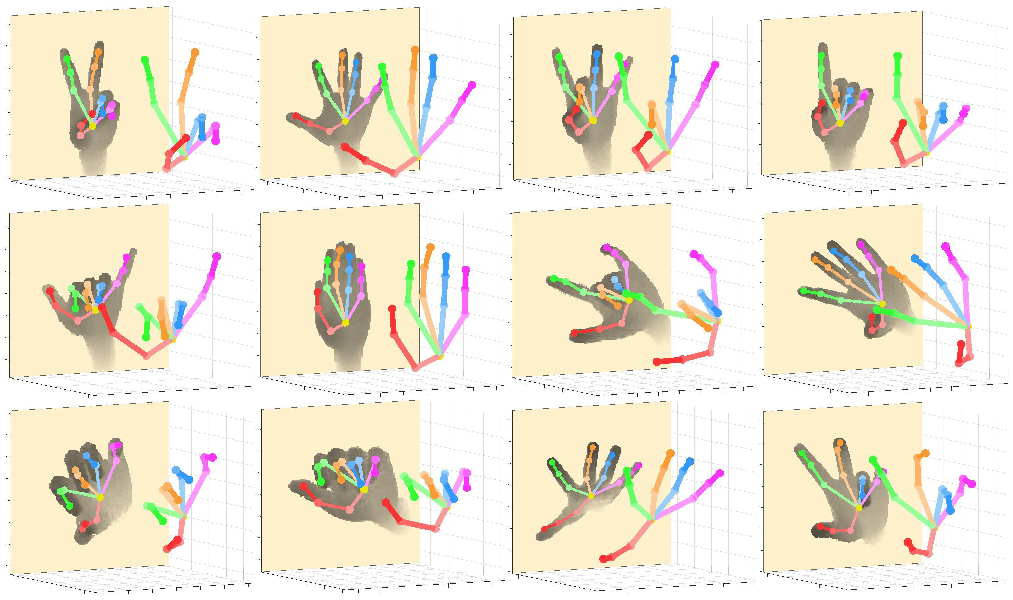
\includegraphics[width=1.0\linewidth]{qualitative_icvl.pdf}
\end{center}
\vspace*{-6mm}
   \caption{Qualitative results of our V2V-PoseNet on the ICVL dataset. Backgrounds are removed to make them visually pleasing.}
\vspace*{-3mm}
\label{fig:qualitative_icvl}
\end{figure*}

\begin{figure*}
\begin{center}
   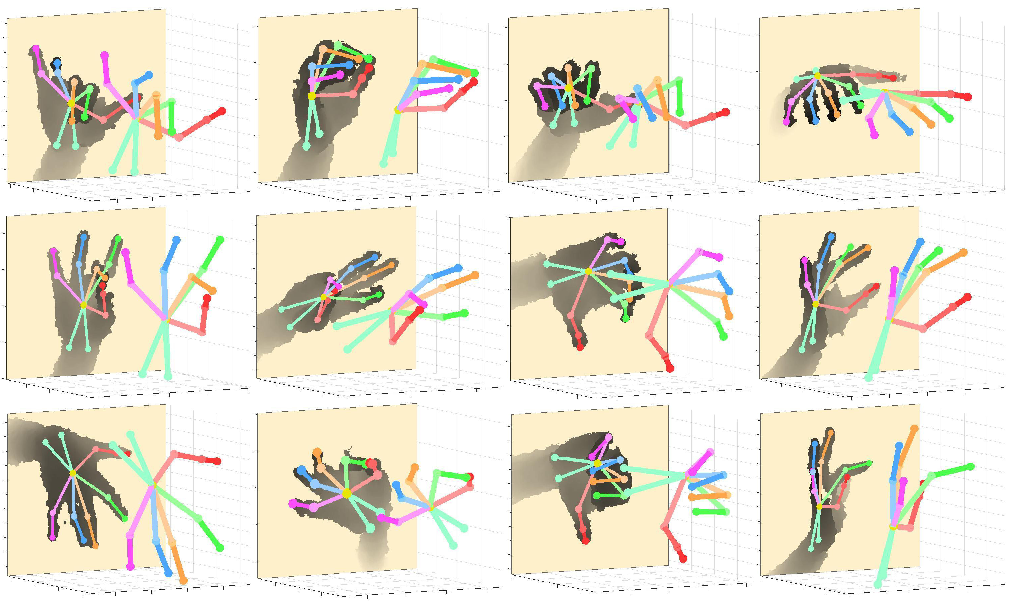
\includegraphics[width=1.0\linewidth]{qualitative_nyu.pdf}
\end{center}
\vspace*{-6mm}
   \caption{Qualitative results of our V2V-PoseNet on the NYU dataset. Backgrounds are removed to make them visually pleasing.}
\vspace*{-3mm}
\label{fig:qualitative_nyu}
\end{figure*}

\begin{figure*}
\begin{center}
   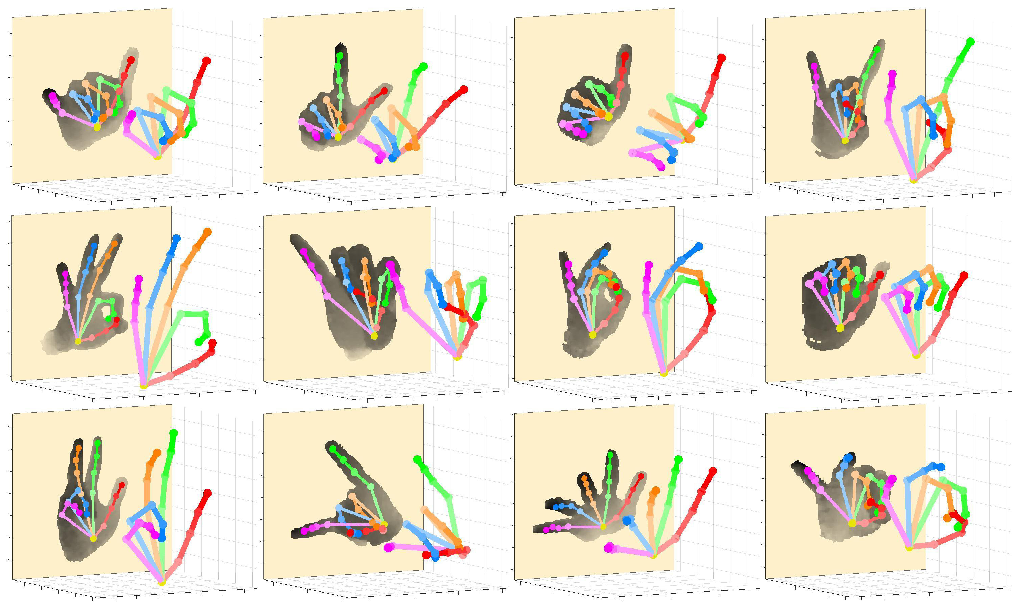
\includegraphics[width=1.0\linewidth]{qualitative_msra.pdf}
\end{center}
\vspace*{-6mm}
   \caption{Qualitative results of our V2V-PoseNet on the MSRA dataset. Backgrounds are removed to make them visually pleasing.}
\vspace*{-3mm}
\label{fig:qualitative_msra}
\end{figure*}

\begin{figure*}
\begin{center}
   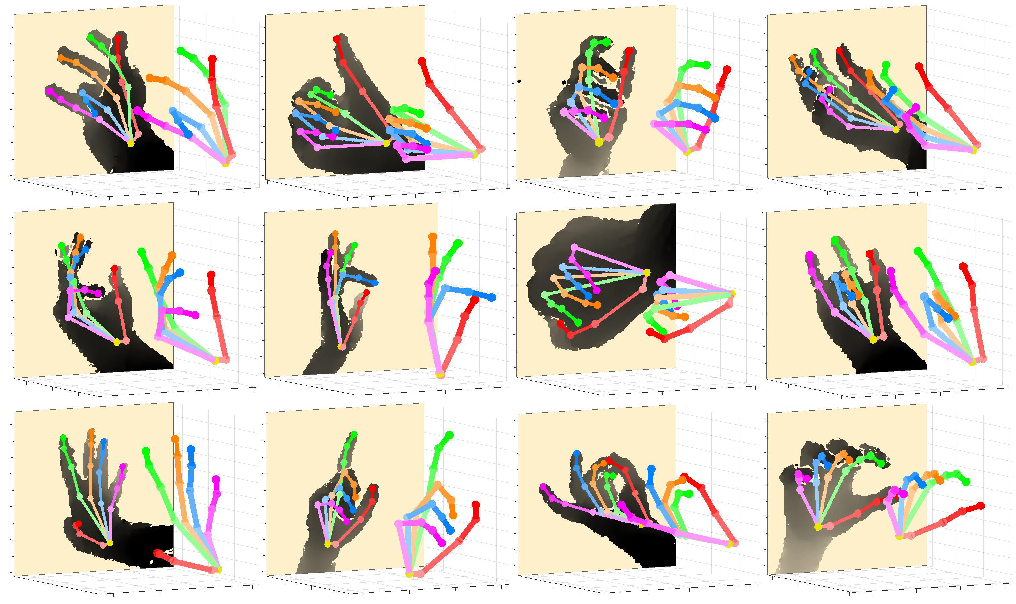
\includegraphics[width=1.0\linewidth]{qualitative_hands2017.pdf}
\end{center}
\vspace*{-6mm}
   \caption{Qualitative results of our V2V-PoseNet on the HANDS 2017 frame-based 3D hand pose estimation challenge dataset. Backgrounds are removed to make them visually pleasing.}
\vspace*{-3mm}
\label{fig:qualitative_hands2017}
\end{figure*}

\begin{figure*}
\begin{center}
   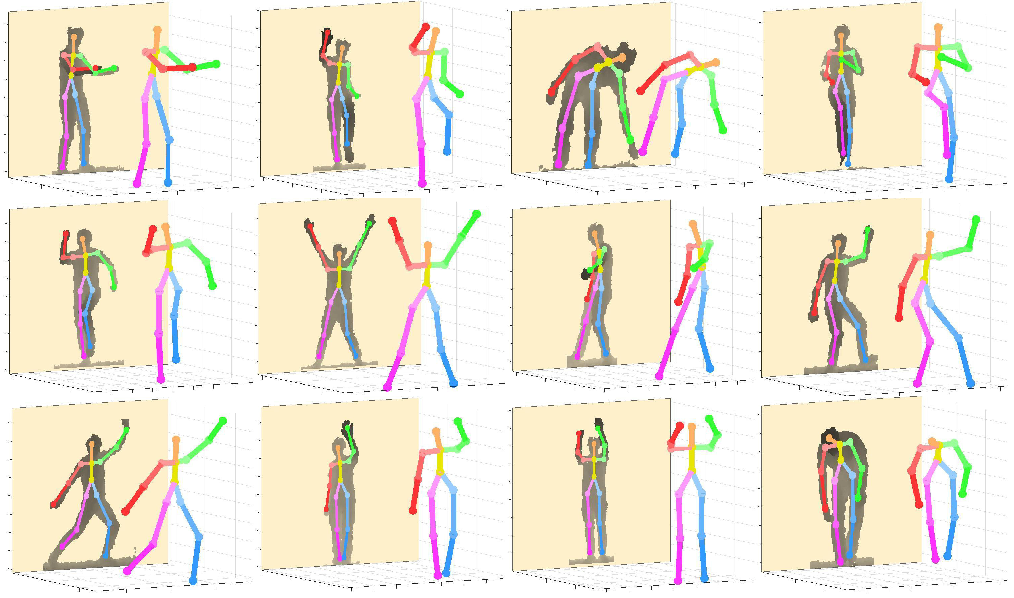
\includegraphics[width=1.0\linewidth]{qualitative_itop_front.pdf}
\end{center}
\vspace*{-6mm}
   \caption{Qualitative results of our V2V-PoseNet on the ITOP dataset (front-view). Backgrounds are removed to make them visually pleasing.}
\vspace*{-3mm}
\label{fig:qualitative_itop_front}
\end{figure*}

\begin{figure*}
\begin{center}
   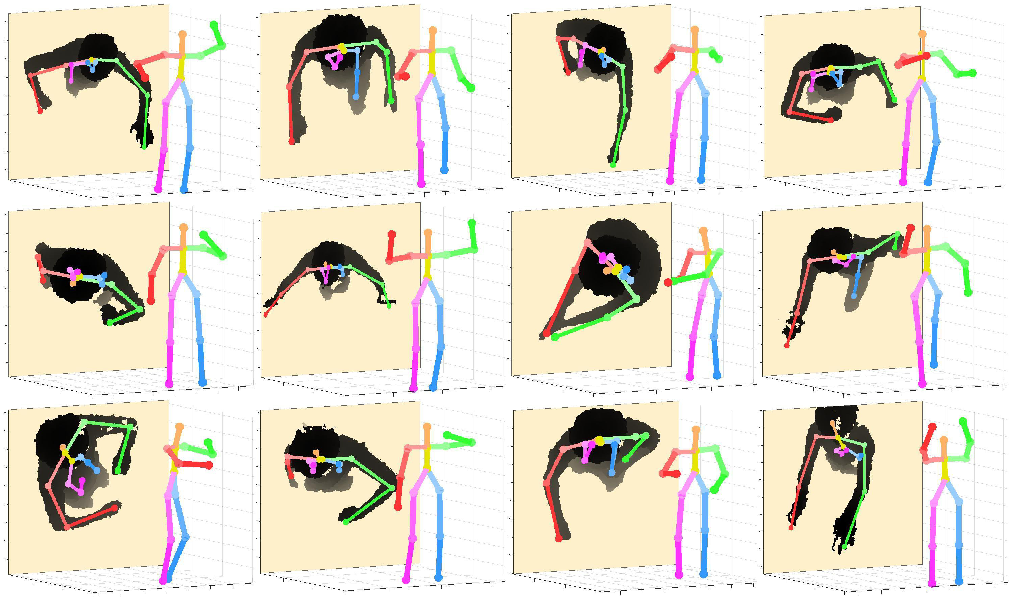
\includegraphics[width=1.0\linewidth]{qualitative_itop_top.pdf}
\end{center}
\vspace*{-6mm}
   \caption{Qualitative results of our V2V-PoseNet on the ITOP dataset (top-view). Backgrounds are removed to make them visually pleasing.}
\vspace*{-3mm}
\label{fig:qualitative_itop_top}
\end{figure*}